% ======================================================= %
% Document: RESPONSE TO REVIEWERS
% Template source: Andrea Ballatore / Eduard Szöcs template,
%   as adapted in POAR_range_limits_AmNat_RESPONSE.tex
% ======================================================= %
\documentclass[12pt]{article}

% If/when a marked-up revised manuscript file exists, point \externaldocument
% at it (without the .tex extension) so that \ref{ms-...} labels below will
% resolve to real line numbers, e.g.:
 \usepackage{xr}
 \externaldocument[ms-]{EcolLett_R1}

\usepackage{graphicx}
\usepackage{url}
\usepackage[usenames,dvipsnames]{xcolor}
\usepackage{color}
\definecolor{mygray}{gray}{0.6}
\usepackage[utf8]{inputenc}
\usepackage[onehalfspacing]{setspace}
\usepackage[
	round,	% round parentheses
	colon,	% separate multiple citations with colons
	authoryear,% author-year citations
	sort,	% order multiple citations into the sequence in which they appear
]{natbib}
\usepackage[%disable
	]{todonotes}

\usepackage{anysize}
\marginsize{2.5cm}{2.5cm}{1.5cm}{2.5cm}

% macros
\newcounter{cN}
\setcounter{cN}{0}

\newcommand{\comment}[1]{
	\vspace{2em}
	\refstepcounter{cN} % increment counter
	\noindent \hangindent=0em \textbf{\textcolor{Maroon}{\uline{Comment \thecN}:~}}\emph{``#1''}
	}

\newcommand{\response}[1]{
	\\[0.25em]
	\hangindent=2.3em \textbf{\textcolor{NavyBlue}{\uline{Response}:~}}#1
	}

\newcommand{\revise}[1]{{\color{Mahogany}{#1}}}

% ulem.sty is unavailable in this build environment; \uline is only used
% here for simple underlining, so provide a minimal shim with base LaTeX's
% \underline instead of loading the package.
\providecommand{\uline}[1]{\underline{#1}}
\definecolor{darkred}{rgb}{1,.6,.6}
\setcounter{secnumdepth}{-1}

\begin{document}
\vspace*{-2em}
\begin{center}
{\LARGE\bfseries Manuscript 7613110 --- Response to reviewers}
\end{center}
\vspace{1em}
% ======================================================= %
\noindent To the editorial board,

Thank you for the opportunity to submit a revision of our manuscript, ``Aridity and herbivory shape demographic benefits of fungal endophytes in cool-season grasses,'' for your consideration. Our major changes include the following:
\begin{enumerate}
	\item {We revised our conceptual framing to incorporate more recent extensions of the stress-gradient hypothesis (SGH), which recognize that positive interactions can weaken or reverse under sufficiently severe or compounding stress, rather than increasing monotonically with stress as in the classic SGH. This revision spans the Introduction (hypotheses), Discussion, and clarifies that our finding of declining endophyte benefits with increasing aridity reflects this more nuanced framework rather than a simple contradiction of SGH (Reviewers 1 \& 2).}
	\item {We conducted a new sensitivity analysis excluding the two field sites (KER and SON) affected by an exclusion-cage disturbance and replanting event, to directly test whether this disturbance or the associated variability in herbivore-exclusion efficacy influenced our results. Posterior estimates of endophyte effects were nearly identical with and without these sites across all species, vital rates, and treatments, and we have added this analysis, along with a new supplementary figure and table, to the manuscript (Reviewer 1).}
	\item {We expanded the Discussion to address the broader biological implications of our results, including the potential consequences of climate-driven shifts in symbiosis costs and benefits for endophyte prevalence, host-range dynamics, and symbiont retention, as well as the role of variation in endophyte alkaloid chemistry in explaining species-specific herbivory responses (Reviewers 1 \& 3). We also corrected a data-interpretation error in the reported herbivory results for \textit{A. hyemalis} (Reviewers 1 \& 3).}
\end{enumerate}

We describe these and other changes in greater detail below, where we reproduce comments from the reviewers and provide our point-by-point responses.
All of our changes are denoted in the manuscript with \revise{Mahogany font}.
We think the review process has strengthened our manuscript and hope you agree that it is now suitable for publication.

\vspace{2em}
\hfill On behalf of myself and coauthors,

\hfill Jacob Moutouama
\newpage

% ======================================================= %
\section{Response to Reviewer 1}
\vspace{-2em}

\comment{The authors test how the benefits of an endophyte symbiosis interacted with climatic stress (precipitation) gradient. They found that the benefits were largely lost with increasing aridity. This is a very strong study that was well designed and the analyses were well interpreted. The results are not entirely novel due to the well documented variation in endophyte benefits depending on the host and endophyte species. Even though the results are not novel, the study is one of the most complete analyses of the relationship between climate and endophyte effects on vital rates under field conditions. I believe this study is a solid contribution to the literature on plant microbial symbiosis. It is also a very well written manuscript.}
\response{We thank Reviewer 1 for these positive and constructive comments. We appreciate the recognition of the study’s experimental design, analytical approach, and contribution to the literature on plant–microbial symbiosis. We agree that variation in the benefits of endophyte symbiosis among host and endophyte species has been well documented. We believe that our study extends this literature by explicitly testing how climatic stress modifies endophyte effects on multiple plant vital rates across a broad precipitation gradient under field conditions. This integrative approach provides a more comprehensive assessment of how climate may shape the demographic consequences of plant–microbial symbioses.}

\comment{The introduction establishes potential costs of symbiosis increasing with stress, but the authors' hypotheses ignore this potential. I think it would be helpful to explain why the authors focused on only hypotheses that were majority beneficial before the hypotheses were established.}
\response{We thank Reviewer 1 for pointing out this issue. We agree that our original presentation did not sufficiently explain why our hypotheses were framed primarily around conditions under which endophyte symbiosis provides demographic benefits, despite acknowledging that the costs of maintaining symbionts may increase with environmental stress. Our intention was not to assume that increasing stress necessarily strengthens mutualism, but rather to test whether the well-documented benefits of \emph{Epichloë} symbiosis are maintained, enhanced, or eroded across environmental conditions. We have therefore clarified this rationale in the Introduction and revised the climate-dependent hypothesis to explicitly recognize that endophyte benefits may weaken or become negative when environmental stress is sufficiently severe for the costs of maintaining the association to outweigh its benefits. We also clarify that the possibility of reduced or reversed benefits under compounded stress is incorporated into our herbivory--climate-dependent hypothesis (line \ref{ms-endocost}).}

\comment{In the methods section, it would be helpful to include some of the past research on these hosts plant species. Have past studies found that these species largely benefit from the endophyte presence? A brief review of the past results would help the reader understand the expectations.}
\response{We thank Reviewer 1 for this helpful suggestion. We have added a brief review of past research on these host--endophyte associations to the Study system section of the Methods (line \ref{ms-hostbenefits}), noting that prior work generally reports beneficial effects of endophyte presence on host performance, though the magnitude and direction vary among host species, vital rates, and environmental conditions. This context supports our expectation of predominantly beneficial effects and motivates our focus on how these benefits shift with aridity. The added text reads:
\begin{quote}
``Previous studies of these associations have generally found beneficial effects on host performance, although effects can vary among host species, vital rates, and environmental conditions \citep{yule2013costs,davitt2011understanding,gundel2020simulated}.''
\end{quote}
}

\comment{Given the results that endophytes benefit the host only under more mesic conditions, I am left wondering, what are the implications of these results for the symbiosis? Does the proportion of symbiotic hosts decline at the drier ends of the spectrum? I would recommend that the authors touch on some of these biological implications.}
\response{We thank Reviewer 1 for highlighting this important biological implication. We agree that the stronger demographic benefits of endophytes under mesic conditions raise the possibility that the balance of costs and benefits could influence the persistence and distribution of the symbiosis across environmental gradients. We have expanded the Discussion to address this implication. Specifically, we now discuss the possibility that if endophyte-associated costs reduce host or symbiont fitness under dry conditions, endophyte prevalence could decline toward the dry end of environmental gradients. We emphasize, however, that this is a prediction arising from our demographic results that requires direct testing through studies of endophyte prevalence and transmission across environmental gradients (line \ref{ms-prevalence}).}

\comment{The conclusion states that the endophyte cannot be expelled from the host and this may have implications for the stress gradient hypothesis; however, there is evidence of imperfect transmission of endophytes between tillers. How may this affect the results of the study? Did the authors test the final proportions of symbiont hosts?}
\response{We thank Reviewer 1 for pointing out this important nuance. We agree that our original statement that vertically transmitted endophytes ``cannot be expelled'' was too absolute. We have revised the sentence to clarify that, although \textit{Epichloë} endophytes are tightly integrated with their hosts and cannot be readily removed from individual host tissues as conditions deteriorate, imperfect transmission provides a potential pathway for symbiont loss over longer timescales. We now explicitly discuss how such transmission dynamics could influence the prevalence and persistence of the symbiosis when the costs of infection increase under stressful conditions (line \ref{ms-transmission}).}

\comment{179--181: How did the destruction of these exclusions affect the results? Were these effects included in the models? Given the high variability of the exclusion efficacy (Figure S3), it would be helpful to provide more detail on the implications of the replanting and any effects on the results.}
\response{We thank Reviewer 1 for raising this important point. Because demographic responses were calculated between consecutive censuses, observations from the replanted KER and SON plots were treated as new $t$--$t+1$ demographic intervals rather than excluded outright, so the disturbance itself does not introduce missing or miscoded transitions (line \ref{ms-replanting}). To directly test whether this disturbance and replanting -- together with the variability in exclusion efficacy at these sites shown in Figure S3 -- influenced our conclusions, we repeated the complete analyses excluding KER and SON entirely. Posterior estimates of endophyte effects on survival, growth, inflorescence production, and spikelet production were nearly identical between the full dataset and the dataset excluding these two sites across all species, vital rates, and herbivory treatments (Fig.~S6, Table~S6). Across the 66 species $\times$ vital rate $\times$ herbivory $\times$ precipitation-level combinations evaluated, the estimated direction of the endophyte effect was unchanged in 65/66 cases, and the 11 effects with strong posterior support (P($\Delta{>}0$) $>$0.95 or $<$0.05) in the full-data analysis retained the same direction and strong support in 10/11 cases when KER and SON were excluded. This indicates that neither the destruction/replanting event nor the associated exclusion-efficacy variability at these sites is driving our main results.
We have added this sensitivity analysis, including the full results (Table~S6) and figure (Fig.~S6) shown above, to the Supplementary Materials, and describe the analysis and its outcome in the Methods (line \ref{ms-replanting}) and Results (line \ref{ms-replantingresults}) of the revised manuscript.}

\begin{minipage}{\linewidth}
\centering
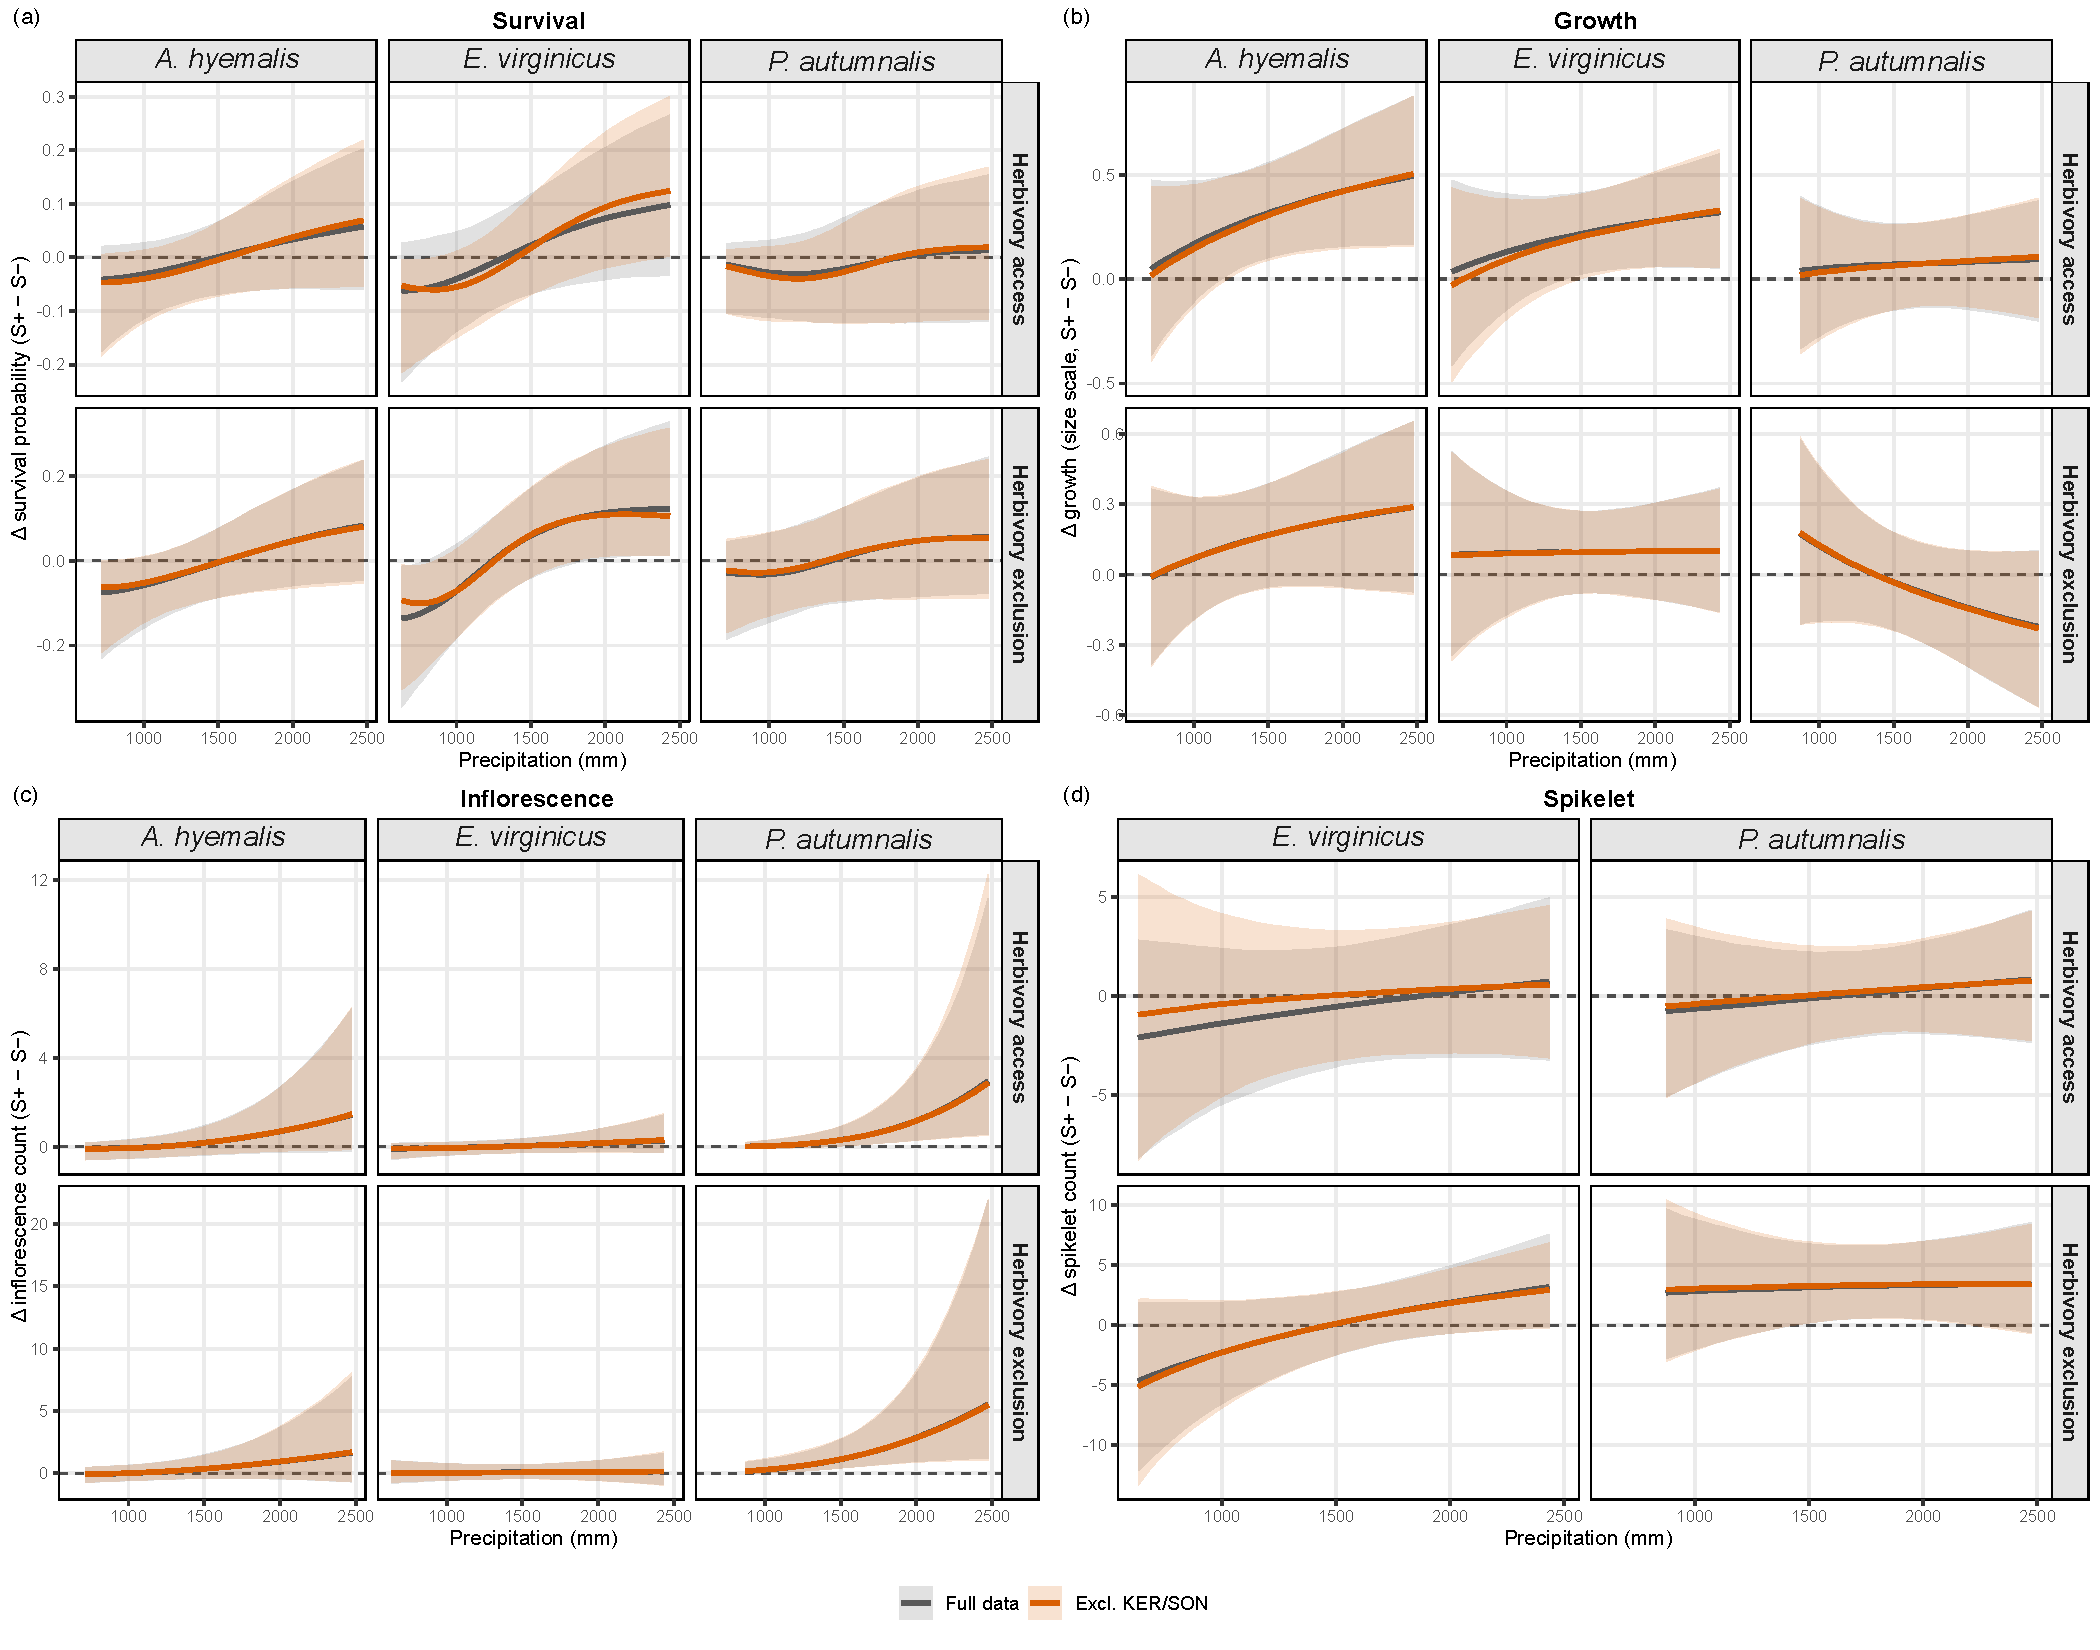
\includegraphics[width=1\linewidth]{FigS_sensitivity_KER_SON_combined.pdf}\\[0.3em]
{Figure S6:Posterior median (line) and 90\% credible interval (shading) of endophyte effects ($\Delta$ = S+ $-$ S-) for the full dataset (gray) and for the dataset excluding KER and SON (orange), by vital rate, species, and herbivory treatment.}
\end{minipage}

\comment{190--193: How were the spikelets for \textit{A. hyemalis} estimated? Table S9 has model results for \textit{A. hyemalis} but not \textit{P. autumnalis}.}
\response{Spikelet counts were not recorded for \textit{A. hyemalis} because its inflorescences contain numerous very small spikelets that are difficult to count reliably in the field. We have clarified in the revised Methods (line \ref{ms-spikeletmethod}) that spikelets were instead counted directly on up to three inflorescences from reproducing individuals of \textit{P. autumnalis} and \textit{E. virginicus}. We also corrected the supplementary table accordingly; the relevant table is now Table S10 and reports spikelet model results for \textit{P. autumnalis} and \textit{E. virginicus} only.}

\comment{220: It may be helpful for clarity to replace ``endo'' with ``symb'' in the model since the test mostly describes the treatment as S+ vs.\ S-.}
\response{We thank Reviewer 1 for pointing out this inconsistency. We have revised the text so that the vital rates are named consistently throughout the manuscript (survival, growth, inflorescence production, and spikelet production), matching the naming used in Fig.~S5. To make the connection between vital rates and model parameters fully explicit, we have also added the complete statistical model to the Methods (line \ref{ms-modeq}), which shows how each vital rate enters the demographic model and defines the associated parameters.}

\comment{276: There appears to be a typo here since \textit{A. hyemalis} appears to experience more herbivore damage by percentage when S+.}
\response{We thank Reviewer 1 for catching this error. The values for \textit{A. hyemalis} were inadvertently misinterpreted in the text. We have corrected the sentence in the revised manuscript (line \ref{ms-herbivoryresults}) to accurately report that $S+$ hosts experienced 19\% herbivore damage compared with 15\% for $S-$ hosts, and revised the interpretation accordingly.}

\comment{310: Cite the figure or table with the spikelet results.}
\response{We thank Reviewer 1 for catching this error. The values for \textit{A. hyemalis} were inadvertently misinterpreted in the text. We have corrected the sentence in the revised manuscript (line \ref{ms-herbivoryresults}) to accurately report that $S+$ hosts experienced 19\% herbivore damage compared with 15\% for $S-$ hosts, and revised the interpretation accordingly.}

\comment{Figure 1. It is hard to read the y-axis S+ versus S-. Would it be possible to not make them superscript or increase the size?}
\response{We thank Reviewer 1 for this helpful suggestion. We have revised Figure 1 to improve the readability of the $S+$ and $S-$ labels by increasing their size and presenting them as regular text rather than superscript.}

\section{Response to Reviewer 2}
\vspace{-2em}

\comment{This manuscript presents results of a field experiment that tests predictions of the classic stress gradient hypothesis (SGH) in plant-endophyte systems. Strengths of this study include testing of clear and biologically interesting hypotheses, rigorous field experiments and statistical analyses, and inclusion of a small complementary greenhouse study to test one particular mechanism that might have confounded their field study findings. Notably, results challenge the predictions of the classics SGH, and the authors propose several explanations for this contradictory finding in the discussion. My main criticism is that the framework for this study seems somewhat over-simplified. There has been substantial work since the original SGH that adds nuance to this concept, especially that SGH predictions may change under extreme or compounding stressors such that positive interactions should increase with decreasing environmental severity (e.g., see Michalet et al.\ 2006, Kawai and Tokeshi 2007, le Roux and McGeoch 2010). These ideas are not mentioned in the introduction at all and only mentioned indirectly in the discussion. Otherwise, this is a strong, well-written study that should be of broad interest to ecologists interested in positive interactions.}
\response{We thank Reviewer 2 for highlighting this important development of the stress-gradient hypothesis. We agree that our original framing was too narrow in emphasizing the classic prediction of a monotonic increase in positive interactions with increasing stress. We have revised the Introduction to acknowledge that subsequent work has identified important departures from this pattern, including plateaus or declines in facilitation under extreme stress and changes in interaction outcomes when multiple stressors occur simultaneously. Specifically, we now note that the intensity, type, and combination of stressors can determine whether increasing stress strengthens or weakens positive interactions, and we cite Michalet et al.\ (2006), Kawai and Tokeshi (2007), and le Roux and McGeoch (2010) in this context (line \ref{ms-sghnuance}).
We have also revised our framing of the hypotheses to recognize that endophyte benefits may weaken or become negative when environmental stress becomes sufficiently severe that the costs of maintaining the symbiosis outweigh its benefits. Thus, although our experimental predictions retain the classic SGH as an important benchmark, we now explicitly consider the possibility of declining or reversed benefits under greater environmental stress. 
Finally, we have revised the Discussion to explicitly interpret our results in light of these extensions of the SGH. We now distinguish our departure from the classic monotonic prediction from the broader SGH literature, noting that our finding of declining endophyte benefits with increasing aridity is consistent with the possibility that positive interactions can weaken or reverse under sufficiently severe stress. We also discuss why these extensions may be particularly relevant to symbioses in which hosts have limited flexibility to regulate symbiont load under stress (line \ref{ms-sghdiscussion}). Together, these changes provide a more nuanced conceptual framework for interpreting our finding that endophyte benefits were strongest under mesic rather than arid conditions, without implying that our study directly tests all of the alternative functional forms proposed in the broader SGH literature.}

\comment{One very minor thing to note is that some supplementary figures are not correctly referenced in the text (e.g., line 240 should be Fig.\ S6 instead of S5 and line 277 should be Fig.\ S3 instead of S4).}
\response{We thank Reviewer 2 for carefully checking the supplementary figure references. We have rechecked the manuscript and corrected the supplementary figure citations accordingly (line \ref{ms-ppcsoil}).}

\section{Response to Reviewer 3}
\vspace{-2em}

\comment{This paper reports a study of symbiotic \textit{Epichloe} effects on four vital rates of three grass species over a precipitation gradient in the field, with and without herbivore exclusion. The work is supplemented with greenhouse experiments to test (and exclude) possible effects of soil origin. I will qualify my report with the caveat that I'm not well versed in the statistical methods. I feel that this is a very well planned and executed study, and provides important new, hypothesis driven insight into the grass-\textit{Epichloe} systems specifically, and the principles of symbiosis generally. I have suggestions to improve the manuscript by filling it out with some additional information (especially in Methods), plus some corrections and clarifications.}
\response{We thank Reviewer 3 for the positive assessment of our study and for the detailed and constructive suggestions. We have addressed each of the points raised below and made corresponding revisions to the manuscript.}

\comment{Line 124 and throughout: ``\textit{E. typhina} subsp.\ \textit{poae}'' should be ``\textit{E. poae}'', since it is now recognized as a species distinct from \textit{E. typhina}. (Also, for taxonomic names, don't italicize words or abbreviations such as sp.\ and subsp.)}
\response{We thank Reviewer 3 for noting this taxonomic update. We have revised the manuscript accordingly, replacing \emph{E. typhina} subsp.\ \emph{poae} with \emph{E. poae} throughout and correcting the formatting of taxonomic abbreviations (e.g., ``sp.'' and ``subsp.'') as suggested (line \ref{ms-taxofix}).}

\comment{Line 124: Do not italicize PauTG-1.}
\response{Corrected as suggested (line \ref{ms-taxofix}).}

\comment{Line 127: Disagreement in number: ``stroma'' is singular. The plural is ``stromata''.}
\response{We thank the reviewer for noting this grammatical error. We have corrected ``stroma'' to ``stromata'' where the plural form is intended (line \ref{ms-stroma}).}

\comment{Line 136 and throughout: I think it looks better to use a proper minus sign (or n-dash) instead of a hyphen for designations such as S--. (Also, does this journal use n-dash for ranges?)}
\response{We thank the reviewer for pointing this out. We have replaced the hyphen with a proper minus sign throughout the manuscript for designations such as S$-$. We have also followed the journal's typographical convention of using an en dash for numerical ranges (lines \ref{ms-Sminus1}, \ref{ms-Sminus2}, \ref{ms-Sminus3}, \ref{ms-Sminus4}, \ref{ms-Sminus5}, \ref{ms-Sminus6}, \ref{ms-Sminus7}, \ref{ms-Sminus8}, \ref{ms-Sminus9}, \ref{ms-Sminus10}).}

\comment{Line 137: Should ``five days'' be ``5 d''?}
\response{Thank you for the suggestion. We have retained “five days” rather than “5 d,” as the journal guidelines do not require the abbreviation “d” for days, and we follow the convention of spelling out numbers below 10 in the text.}

\comment{Line 138: Never spell out ``minutes''. The standard unit is ``min''.}
\response{Thank you for the suggestion. We have retained “minutes” to be consistent with the journal guidelines, which request the use of SI units where possible but do not specifically require the abbreviation “min” in running text.}

\comment{Line 142: Give the actual concentration of sodium hypochlorite. Also, the surface sterilization procedure was undoubtedly more involved than stated, so either a full description or reference to it in the literature is needed here.}
\response{\revise{I skip this question to get Tom opinion on this}}

\comment{Line 143: More detail needed here also: what temperature? What light regime?}
\response{\revise{I will do this once I hear back from Tom.}}

\comment{Lines 147--150 (and Table S1): I have a hard time interpreting this and relating it to the experiment as described in the section following. Several questions: What is the operational definition of genotype in this study? How was that diversity established and maintained? What is the relevance of the numbers of genotypes reported here and in Table S1? It seems that, from the information in Lines 174-181 that only a fraction of that genotype diversity was actually utilized in the experiments.}
\response{We thank the reviewer for pointing out this lack of clarity. We have revised the Methods to define “genotype” operationally as an independently collected source individual and its vegetatively propagated descendants, such that clones derived from the same source individual represent the same genetic background (line \ref{ms-genotypedef}). We now clarify that these source genotypes were maintained through vegetative propagation and refer readers to Table S1 for the number of source genotypes and clonal replicates represented in each source population. We have also clarified how these propagated plants relate to the plants included in the experiment (line \ref{ms-genotypedef}). 
%These changes should make the role of genotype and the information presented in Table S1 clearer.
}

\comment{Lines 176--177 ``Each plot was planted with 15 individuals, a mix of S+ and S- plants'': How many of each (S+ vs S--)?}
\response{Thank you for pointing this out. We have clarified the numbers of S+ and S\textminus plants corresponding to each starting endophyte frequency (line\ref{ms-nbind}).}

\comment{Line 189: Should ``on up to three'' be ``on up of three''?}
\response{Thank you for the suggestion. We have retained “on up to three,” as this indicates that spikelets were counted on a maximum of three inflorescences per reproducing individual.}

\comment{Lines 192-193: I'm not sure of the reason for this sentence. I would think it sufficient to state that \textit{A. hyemalis} spikelets were too numerous and small to count (maybe a rephrasing of the previous sentence).}
\response{We have simplified this sentence as suggested (line\ref{ms-spikeletmethod}).}

\comment{Line 193: Change ``while'' to ``whereas''. ``While'' implies simultaneous occurrence. I suggest you check usage of ``while'' throughout the paper. Often a better word in context is although, but, whereas, etc.}
\response{Thank you for the suggestion. We have changed “while” to “whereas” here to make the contrast between species more explicit (line\ref{ms-whereas1}).}

\comment{Statistical modeling section: I think it might help the reader if the name the vital rates and explicitly connect each to the parameters. In Fig S5 the vital rates are named Survival, Growth, Inflorescence and Spikelet. But line 204 lists ``survival, growth, and fertility.'' Some clarification is needed here.}
\response{Thank you for pointing this out. We have clarified the terminology by specifying that fertility was quantified as inflorescence and spikelet production (\ref{ms-vital}).}

\comment{Line 210: Actually, I don't know what the distinction is ``between flowering occurrence and inflorescence production''. Can this be explained?}
\response{We agree that this distinction was not sufficiently clear. We have clarified that the hurdle model distinguishes between whether a plant produced any inflorescences and, conditional on producing inflorescences, how many it produced (line \ref{ms-inflorescence}).}

\comment{Lines 275-276, ``S+ hosts experienced less herbivore damage than S- hosts in \textit{A. hyemalis} (19\% vs.\ 15\%) and \textit{P. autumnalis} (13\% vs.\ 18\%)'': The orders of the numbers given aren't consistent, and would cause me to think that there is more damage on S+ for \textit{A. hyemalis}, but less on S+ for \textit{P. autumnalis}.}
\response{We thank Reviewer 3 for catching this error. The values for \textit{A. hyemalis} were inadvertently misinterpreted in the text. We have corrected the sentence in the revised manuscript (line \ref{ms-herbivoryresults}) to accurately report that $S+$ hosts experienced 19\% herbivore damage compared with 15\% for $S-$ hosts, and revised the interpretation accordingly.}


\comment{Lines 344-345, ``These results contradict predictions\ldots'': Is the contradiction with respect to the abiotic stresses only, or is the herbivore effect also in contradiction of the hypothesis? The context (previous sentence) seems to imply the latter, but I doubt that's what's meant.}
\response{We thank the reviewer for identifying this ambiguity. We agree that our original wording could be interpreted as suggesting that the herbivory results also contradicted the SGH. This was not our intent. Our departure from the classic SGH prediction concerns the abiotic stress gradient, where endophyte benefits declined rather than increased with increasing aridity. In contrast, herbivory effects were inconsistent across species and fitness components, although the strongest effects were in the predicted direction. We have revised the text to make this distinction explicit and to clarify that our results provide mixed evidence for the predicted effects of herbivory (line \ref{ms-sghdiscussion}).
}

\comment{Lines 385-388: It should also be noted that the endophytes typically associated with these grasses may differ strongly in which and how much anti-herbivore alkaloids they have. For example, high levels of the potent anti-insect loline alkaloids (plus low levels of peramine) have been documented in \textit{Poa autumnalis}, whereas \textit{Elymus virginicus} has been found to have chanoclavine (activity unknown) and peramine (a feeding deterrent, not as potent as lolines), and different chemotypes are reported for different \textit{E. amarillans} isolates from \textit{A. hyemalis}. See the cited alkaloid literature, but note that especially for sexual \textit{Epichloe} species such as in \textit{E. virginicus} and \textit{A. hyemalis}, there is likely to be considerable variation. In \textit{Poa autumnalis} (Siegel et al.\ 1990), which has an asexual endophyte, one might expect a consistent alkaloid profile compared to what has been published, but there is no guarantee.}
\response{We thank the reviewer for this important point. We agree that differences among the endophytes in the identity and abundance of anti-herbivore alkaloids could contribute to the species-specific herbivory responses we observed. We have revised the Discussion to acknowledge this possibility and added the relevant literature on alkaloid profiles in the endophytes associated with \textit{P. autumnalis}, \textit{E. virginicus}, and \textit{A. hyemalis}. Because we did not characterize endophyte strains or quantify alkaloid profiles in this study, we now present variation in endophyte chemistry as a potential explanation rather than attributing the observed responses to specific alkaloids. We also retain host condition as a potential explanation for the increased herbivory observed in endophyte-symbiotic \textit{E. virginicus}, but have revised the text to make clear that these mechanisms are not mutually exclusive (line \ref{ms-alkaloid}).}

\comment{Line 403: I didn't see where this was tested. It seems that the underlying assumption was that the S+ plants retained the endophyte throughout the experiment. Were there any data taken on endophyte presence later, such as at the end of the study?}
\response{We thank the reviewer for pointing out this important limitation. We agree that our study did not directly test whether hosts retained their endophytes throughout the experiment, as we did not re-assess endophyte presence at the end of the study. We have therefore revised the Discussion to frame host control over symbiont retention as a potential mechanism rather than a conclusion supported by our data, and we now explicitly acknowledge that we cannot determine whether variation in symbiont retention contributed to the demographic patterns we observed (line \ref{ms-symbiont-retention}).
}

\comment{Lines 417-420: Can the authors comment---even speculate--- on why other studies have found host-range expansion effects of \textit{Epichloe}? Does that have to do with specifically which factors limit the hosts and establish those ``range margins''?}
\response{We thank the reviewer for this insightful suggestion. We agree that whether \textit{Epichloë} expands or constrains host ranges may depend on the environmental factors establishing range margins. We have added this possibility to the Discussion, noting that endophytes may promote range expansion when their benefits offset the factor limiting host performance, but may provide little benefit when the limiting factor is severe resource stress that cannot be alleviated by the symbiosis. This provides a potential explanation for why previous studies have reported host-range expansion effects of \textit{Epichloë}, while our results show declining demographic benefits with increasing aridity (line \ref{ms-range-expansion}).
}

\comment{Figures: In general I think that saturation contrast can be used to better distinguish treatments in line graphs and bar graphs (Fig.\ 1, Fig.\ 2 panels b, d and f, Fig.\ 5, and Fig.\ 6 panel e). In general, I suggest checking readability for common types of color blindness.}
\response{We thank the reviewer for this helpful suggestion. We revised the color palettes across all figures to increase saturation and contrast between treatments and improve visual distinction. We also adopted a consistent cool-toned, colorblind-accessible palette throughout the figures and checked the revised figures for readability under common forms of color-vision deficiency.}

\comment{Fig.\ S2 and S3: I think the bar colors and orders, viz herbivore access vs exclusion, are switched between these two figures. That's confusing. (Also try to match color usage in Figs.\ 1, 5, and S10).}
\response{We have corrected the color/order inconsistency between Figs.\ S2 and S3 and matched color usage across Figs.\ 1, 5, and S10.}

\comment{Figs.\ S5 and S6: What are the axes?}
\response{We thank the reviewer for noting the need for clearer axis labels. We have revised the posterior predictive check figure to explicitly identify the response variable on the x-axis for each vital rate (survival status, growth, inflorescence count, and spikelet count) and to label the y-axis as probability density, which represents the density of the observed and posterior predictive distributions. We also added panel labels (A--D) to facilitate reference to individual vital rates.}

\newpage
%\bibliographystyle{plain}
\bibliographystyle{apalike}
\bibliography{References}
% ======================================================= %
\end{document}
% ======================================================= %
